\documentclass[a4paper,11pt]{article}
\usepackage[utf8]{inputenc}
\usepackage[russian]{babel}
\usepackage[T1]{fontenc}
\usepackage{amssymb,amsmath,graphicx,indentfirst}

\author{Иван Веселов}
\title{Курс kiev-clrs -- Лекция 13. Амортизационный анализ}
\date{2009 г.}

\begin{document}

\maketitle
\tableofcontents
\newpage

\setlength{\parskip}{1ex plus 0.5ex minus 0.2ex}

\section{План лекции}
\begin{itemize}
\item Динамические хэш-таблицы
\item Групповой анализ
\item Метод бухгалтерского учёта
\item Метод потенциалов
\end{itemize}

\section{Динамические таблицы}

\textbf{Вопрос}: насколько большой должна быть хэш-таблица?

Соображения:
\begin{itemize}
\item нам нужно сделать её как можно больше, т.к. с ростом размера таблицы
  уменьшается время поиска
\item нам нужно сделать её как можно меньше, т.к. в противном случае мы тратим
  много памяти на хранение таблицы
\end{itemize}

Таким образом, мы должны соблюдать баланс между временем и памятью. Вспомним,
что время поиска в хэш-таблице равно $O(1 + \alpha)$, где $\alpha$ --
коэффициент заполненности таблицы. Очевидно что оптимум достигается, если
$\alpha$ -- константа, т.е. $\alpha = n/m = O(1) \Rightarrow m = O(n)$. Мы
получили, что оптимальным решением для размера таблицы будет $\Theta(n)$ для $n$
ключей.

\textbf{Задача}: Но что делать если мы не знаем $n$ наперёд?

\textbf{Решение}: использовать динамические хэш-таблицы!

\textbf{Идея}: когда таблица ``переполняется'' (в ней становится слишком много элементов)
-- мы увеличиваем её размер (например вдвое):

\begin{enumerate}
\item выделяем (malloc или new) место для большей таблицы
\item перемещаем элементы из старой таблицы в новую
\item освобождаем память, занимаемую старой таблицей
\end{enumerate}

\begin{figure}[ht]
  \centering
  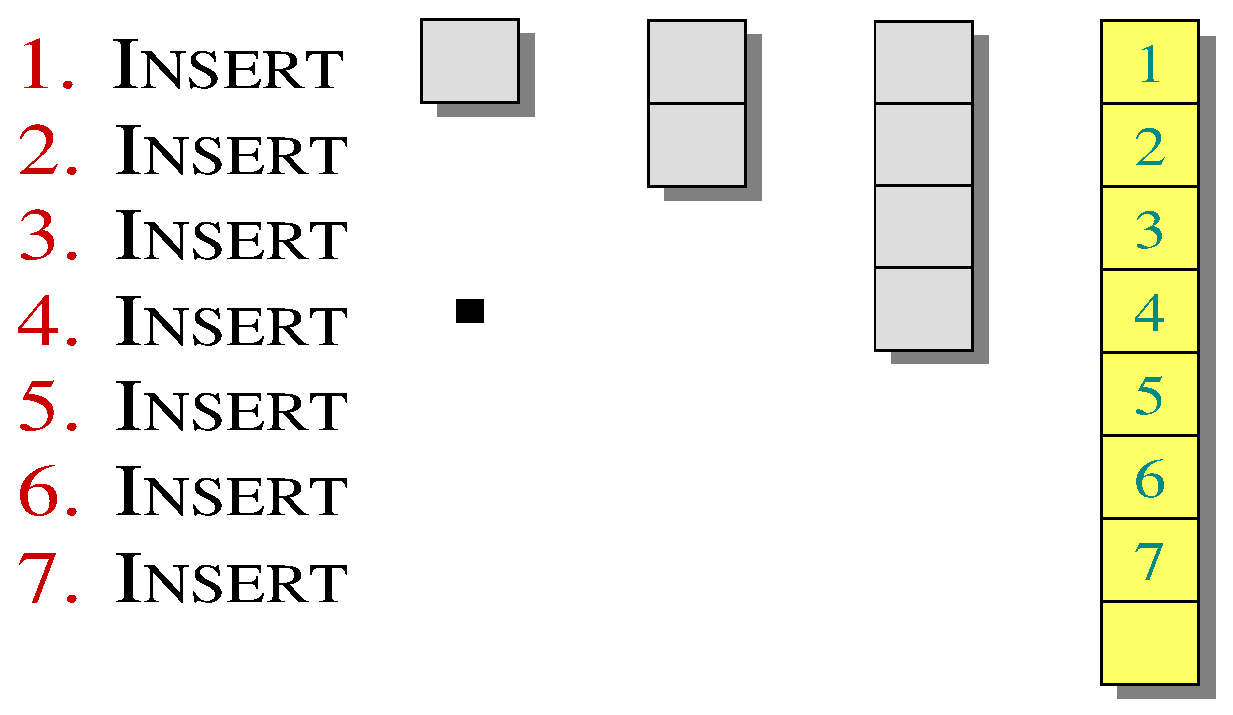
\includegraphics[width=3in]{lecture13/insertion.eps}
  \caption{Пример заполнения динамической таблицы}
  \label{fig:insertion}
\end{figure}

Проведём анализ наихудего случая в таком алгоритме:

\begin{itemize}
\item анализируем последовательность из $n$ операций
\item каждая операция выполняется максимум за время $O(n)$.
\end{itemize}

Значит ли это, что вся последовательность выполняется за $O(n^2)$?

Нет, такой анализ был бы неточным. На самом деле последовательность из $n$
операций выполняется за время $O(n) << O(n^2)$.

Покажем почему. Пусть $c_i$ -- стоимость $i$-й операции.
$$
c_i = 
\begin{cases}
  i, \text{ если } i - 1 \text{ -- степень двойки}\\
  1, \text{ в противном случае}
\end{cases}
$$

\begin{center}
\begin{tabular}{|r|c|c|c|c|c|c|c|c|c|c|}
  \hline
     $i$ & 1 & 2 & 3 & 4 & 5 & 6 & 7 & 8 & 9  & 10 \\
  \hline
$size_i$ & 1 & 2 & 4 & 4 & 8 & 8 & 8 & 8 & 16 & 16 \\
  \hline
   $c_i$ & 1 & 2 & 3 & 1 & 5 & 1 & 1 & 1 & 9  & 1 \\
  \hline
   $c_i$ & 1 & 1 & 1 & 1 & 1 & 1 & 1 & 1 & 1 & 1 \\
         & 0 & 1 & 2 & 0 & 4 & 0 & 0 & 0 & 8 & 1 \\
  \hline
\end{tabular}
\end{center}

Стоимость $n$ операций равна:
$$
\sum_{i=1}^n c_i = n + \sum_{j=0}^{\lfloor \lg(n - 1) \rfloor} 2^j \leqslant n +
2n = 3n = \Theta(n)
$$

Таким образом среднее время выполнения одной операции $\Theta(n) / n =
\Theta(1)$, а не $\Theta(n)$.

Несмотря на то, что некоторые из операций могут быть трудоёмкими, их немного и
их стоимость распределяется по остальным, менее трудоёмким операциям, таким
образом образую хорошую среднюю оценку времени выполнения.

При \emph{амортизационном анализе} время, требуемое для вполнения
последовательности операций над структурой данных, усредняется по \emph{всем}
выполняемым операциям. Этот анализ можно использовать, например, чтобы показать,
что даже если одна из операций является дорогостоящей, то при усреднении по всей
последовательности средняя стоимость операций будет небольшой. Амортизационный
анализ отличается от анализа средних величин тем, что в нём не учитывается
вероятность. При амортизационном анализе гарантируется \emph{средняя
производительность операций в наихудшем случае}.

Три метода проведения амортизационного анализа:

\begin{itemize}
\item групповой анализ (aggregate analysis)
\item метод бухгалтерского учёта (accounting method)
\item метод потенциалов (potential method)
\end{itemize}

Групповой анализ мы только что увидели. В процессе группового анализа
показывается, что в наихудшем случае времия выполнения $n$ операций равно $T(n)$.
Поэтому средняя амортизированная стоимость одной операции равна $T(n)/n$. Этот
метод прост, однако уступает другим методам в точности, поскольку не делает
различия между операциями, присваивая всем операциям (даже разнотипным) равную
амортизированную стоимость.

\section{Метод бухгалтерского учёта}

В этом методе разные по типу операции оцениваются различной стоимостью в
зависимости от фактической стоимости. Величина, которая начисляется на операцию
$i$ называется амортизированной стоимостью $\hat{c}_i$. Если начисленная
стоимость превышает фактическую, то остаток рассматривается как ``кредит'' и
присваивается определённым элементам структуры данных. Кредит может в дальнейшем
использоваться для погашения стоимости более дорогостоящих операций, для оплаты
которых не хватает начисляемой амортизированной стоимости.

Рассмотрим общую схему метода:

\begin{itemize}
\item наделить каждую операцию определённой амортизационной стоимостью
  $\hat{c}_i$. Пускай 1 гр. будет платой за определённую единицу работы.
\item при выполнении операции мы тратим её фактическую стоимость $c_i$
\item не потраченный остаток может быть сохранён в банке (в элементе структуры
  данных) для дальнейшего использования
\item общий баланс должен оставаться положительным, т.е.
$$ \forall{n}: \sum_{i=1}^n c_i \leqslant \sum_{i=1}^n \hat{c}_i $$
\item таким образом, суммарная амортизационная стоимость определяет верхнюю
  границу для суммарной фактической стоимости
\end{itemize}

Проведём анализ методом бухгалтерского учёта на примере динамической
хэш-таблицы.

Начислим на $i$-ю операцию вставки стоимость $\hat{c}_i = 3$ гр.
\begin{itemize}
\item 1 гр. тратится непосредственно на вставку (на каждом шаге)
\item 2 гр. сохраняются в ячейке для последующего использования при удваивании
  размера таблицы
\item когда таблица удваивается -- то последние ячейки (с двумя гривнами)
  оплачивают траты на своё копирование и на копирование одной из более старых ячеек.
\end{itemize}

\begin{figure}[ht]
  \centering
  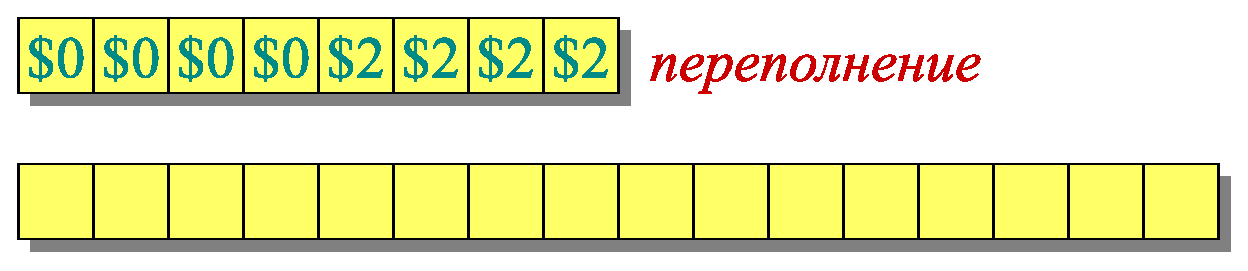
\includegraphics[width=3in]{lecture13/accountant1.eps}
  \caption{Состояния перед удваиванием таблицы}
  \label{fig:acc1}
\end{figure}

\begin{figure}[ht]
  \centering
  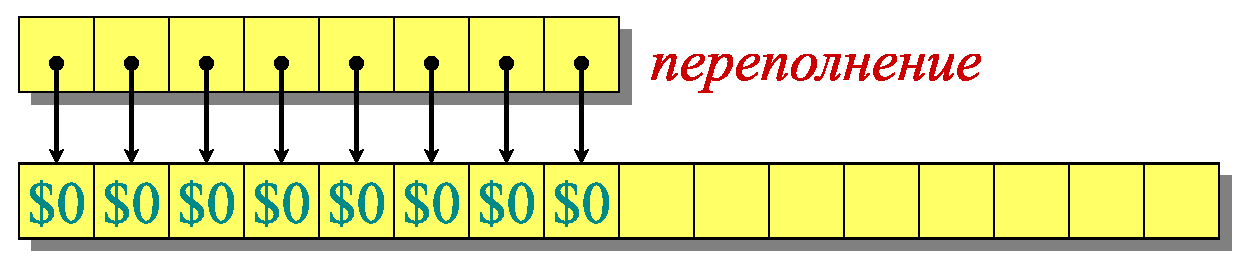
\includegraphics[width=3in]{lecture13/accountant2.eps}
  \caption{Копирование ячеек}
  \label{fig:acc2}
\end{figure}

\begin{figure}[ht]
  \centering
  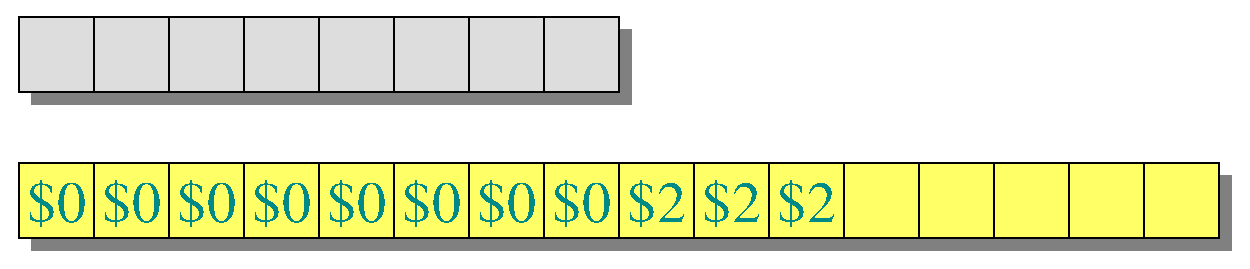
\includegraphics[width=3in]{lecture13/accountant3.eps}
  \caption{После удваивания таблицы}
  \label{fig:acc3}
\end{figure}

Добавим в нашу таблицу значения амортизированной стоимости:

\begin{center}
\begin{tabular}{|r|c|c|c|c|c|c|c|c|c|c|}
  \hline
      $i$ & 1 & 2 & 3 & 4 & 5 & 6 & 7 & 8 & 9  & 10 \\
  \hline
 $size_i$ & 1 & 2 & 4 & 4 & 8 & 8 & 8 & 8 & 16 & 16 \\
  \hline
    $c_i$ & 1 & 2 & 3 & 1 & 5 & 1 & 1 & 1 & 9  & 1 \\
  \hline
    $c_i$ & 1 & 1 & 1 & 1 & 1 & 1 & 1 & 1 & 1 & 1 \\
          & 0 & 1 & 2 & 0 & 4 & 0 & 0 & 0 & 8 & 1 \\
  \hline
$\hat{c}_i$ & $2^*$ & 3 & 3 & 3 & 3 & 3 & 3 & 3 & 3 & 3 \\
  \hline
   $bank_i$ & 1 & 2 & 2 & 4 & 2 & 4 & 6 & 8 & 2 & 4 \\  
  \hline
\end{tabular}
\end{center}

Соблюдается инвариант: баланс в банке никогда не меньше нуля, соответственно
амортизированные стоимости определяют верхнюю границу для фактических
стоимостей. Получаем границу в $\Theta(n)$.


\section{Метод потенциалов}

Идея: структура данных обладает некоей характеристикой, которая называется
потенциалом (из физики). Потенциал -- возможность выполнять работу, то есть
операции над структурой данных (опять же аналогия с физикой: потенциальная
энергия).

Рассмотрим структуру данных, которая изменяется под воздействием
последовательности $n$ операций, обозначим её начальное состояние $D_0$, а
состояние после воздействия $i$-й операции -- $D_i$. Кроме того введём функцию
$\Phi$, которая отображает множество состояний $D$ в множество действительных
чисел $\mathbb{R}$. Эта функция и определяет потенциал структуры данных. Принято
выбирать такую $Phi$, что

$$
\Phi(D_0) = 0, \forall i: \Phi(D_i) \geqslant 0
$$

При таких обозначениях амортизированная стоимость $i$-й операции определяется
как:

$$
\hat{c}_i = c_i + \underbrace{\Phi(D_i) - \Phi(D_{i-1})}_{\text{разница } \Delta \Phi_i}
$$

Возможны два варианта: амортизированная стоиость операции может быть больше или
меньше чем фактическая стоимость:

\begin{itemize}
\item $\Delta \Phi_i > 0$ -- т.е. $\hat{c}_i > c_i$ и эта операция накапливает
  потенциал на следующие, более дорогостоящие операции
\item $\Delta \Phi_i < 0$ -- т.е. $\hat{c}_i < c_i$ и эта операция является
  дорогостоящей и использует ранее накопленный потенциал для выполнения работы
\end{itemize}

Подсчитаем суммарную амортизационную стоимость:
\begin{gather*}
\sum_{i=1}^n \hat{c}_i = \sum_{i=1}^n (c_i + \Phi(D_i) - \Phi(D_{i-1})) = \\
= \text{ (поскольку ряд телескопический) } = \\
= \sum_{i=1}^n c_i + \Phi(D_n) - \Phi(D_0) \geqslant \\
\geqslant \sum_{i=1}^n c_i \text{ (т.к. } \Phi(D_0) = 0 \text { и } \Phi(D_n)
\geqslant 0 \text{) }
\end{gather*}

Таким образом получаем, что амортизационная оценка по методу потенциалов
является верхней границей для суммарной фактической стоимости.

Проанализируем методом потенциалов вставку в динамическую таблицу.

Начинать анализ следует с определения потенциальной функции $\Phi$, сделать это
можноо, например, базируясь на нашей предыдущей идее для метода бухггалтерского
учёта и подсчитав суммарное количество кредитов в зависимости от количества
хранимых ячеек. Таким образом

$$
\Phi(D_i) = 2i - 2^{\lceil \lg n \rceil}
$$

Предполагая, что $2^{\lceil \lg 0 \rceil} = 0$, получим что $\Phi(D_0) = 0$.
Также очевидно, что $\Phi(D_i) \geqslant 0$, поскольку $2^{\lceil \lg i \rceil}
\leqslant 2^{\lg i + 1} = 2i$. Таким образом базовые свойства потенциальной
функции выполняются. 

\begin{figure}[ht]
  \centering
  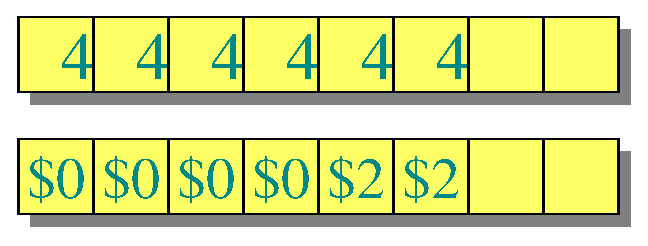
\includegraphics[width=2in]{lecture13/potentials.eps}
  \caption{Потенциальная функция $\Phi = 2 \cdot 6 - 2^3 = 4$}
  \label{fig:potentials}
\end{figure}

Амортизационная стоимость $i$-й операции:

$$
\hat{c}_i = c_i + \Phi(D_i) - \Phi(D_{i-1}) = 
\begin{cases}
  i \text{ если } i - 1 \text { точная степень двойки} \\
  1 \text{ в противном случае }
\end{cases} + 
$$

\begin{gather*}
+ (2i - 2^{\lceil \lg i \rceil})
+ (2(i-1) - 2^{\lceil \lg (i-1) \rceil}) =\\
= \lbrace \cdots \rbrace + 2 - 2^{\lceil \lg i \rceil} + 2 ^{\lceil \lg (i-1)
  \rceil}
\end{gather*}

В зависимости от того, каким образом соотносятся потолки $\lg i$  и $\lg(i-1)$
мы получаем два случая:

\begin{itemize}
\item $i - 1$ -- точная степень двойки, тогда потолки различаются и разница не
  будет равна нулю:
  \begin{align*}
    \hat{c}_i &= i + 2 + 2 - 2^{\lceil \lg i \rceil} + 2 ^{\lceil \lg (i-1)  \rceil} \\
    &= i + 2 - 2(i - 1) + (i - 1) \\
    &= i + 2 - 2i + 2 + i - 1 \\
    &= 3
  \end{align*}
\item $i - 1$ -- не точная степень двойки, тогда потолки не различаются и разница
  будет равна нулю:
  \begin{align*}
    \hat{c}_i &= 1 + 2 - 2^{\lceil \lg i \rceil} + 2 ^{\lceil \lg (i-1)  \rceil} \\
    &= 3
  \end{align*}
\end{itemize}

Таким образом, амортизированная стоимость константна и значит последовательность
$n$ вставок выполняется за время $\Theta(n)$.

\section{Заключительные замечания}

\begin{itemize}
\item методы потенциалов и бухгалтерского учёта похожи и могут быть легко
  трансформированы друг в друга. Они обладают равной мощностью и
  выразительностью, несмотря на то, что в методе бухгалтерского учёта мы
  обладаем дополнительной информацией о расположении кредитов по элементам.
\item в процессе анализа возможны присваивания различных амортизационных
  стоимостей операциям, при этом варианты могут отличаться, давать разные
  оценки, но быть одновременно верными.
\end{itemize}

\end{document}

